\section{Developer Documentation}
\label{sec:devdocs} 

\subsection{Prerequisites}

In order to do development work on \emph{Colonizers}, the following software
is required:
\begin{itemize}
    \item .NET Core 3.1 SDK
    \item Python 3.7 (NOTE: there is an issue if you are using the embeddable
        version of Python, please refer to \Cref{dd:embedpy} for more information)
    \item Node.js 10 and NPM 6.4.1
\end{itemize}
The game's UI is designed for a minimum screen resolution of 1920x1080 at
100\% zoom level. It is not recommended to play the game on lower resolution
screens, since graphical errors may occur.

In order to build and run \emph{Colonizers} in Electron, the Electron.NET CLI
package is required. You may install this package as a .NET Core tool by running
the \texttt{dotnet tool install ElectronNET.CLI -g} command. This gives you
access to the \texttt{electronize} command.

It is also highly recommended to use Visual Studio 2019 for development work
on the game engine or the UI. Visual Studio 2019 provides support for debugging
both the UI and the game engine in the same window, which makes for a~seamless
development experience. Visual Studio 2019 is also capable of attaching
to an external process for debugging, which turns out to be
extremely useful with Electron.NET.

For developing and debugging Python AI scripts, the author used Visual Studio Code,
but other software capable of debugging Python scripts is viable as well.

The project can be run by navigating to the project directory of the \texttt{Desktop} project
and running the command \texttt{electronize start}. This will build the application
and start it inside Electron. Building the application is also done with the
\texttt{electronize} command-line tool. If we want to build \emph{Colonizers}
for Windows 64-bit, we would use the command \texttt{electronize build /target win}.
Further documentation for the \texttt{electronize} command-line tool
is available in the documentation for the Electron.NET project \cite{Electronnet}.
Among other things, the CLI can also produce Win32 builds of the application
with the following command:
\texttt{electronize build /target custom win7-x86;win /electron-arch ia32}.

\subsection{Project Structure}

The entire game is contained in a .sln (solution) file, which is a file type used
to organize projects in Visual Studio. This solution contains five projects:
\begin{itemize}
    \item \texttt{AICore} --- project with the API for AI scripts and the AICore
        scripts themselves.
    \item \texttt{Desktop} --- project with the UI, consisting of an~Angular
        web application and an ASP.NET Core Web API. The Web API is the
        \emph{ClientApp} subdirectory of this project's directory.
    \item \texttt{Game} --- C\# library project containing the game logic
        and code responsible for communicating with Python AIs.
    \item \texttt{Experiments} --- console application project containing
        the experiment scenarios explored in this thesis.
    \item \texttt{ColonizersTests} --- unit test project using xUnit
        as the testing framework. Tests can be run with the command
        \texttt{dotnet test}, or through Visual Studio 2019's test explorer.
\end{itemize}

The flow of data in the application starts with the UI, since all initiative starts
with the user. The UI then uses the ASP.NET Core Web API to execute game logic.
If required, game logic then talks to processes executing Python AI scripts.
This flow can be seen in \Cref{dd:sequence}.

\begin{figure}[ht]
\centerline{\mbox{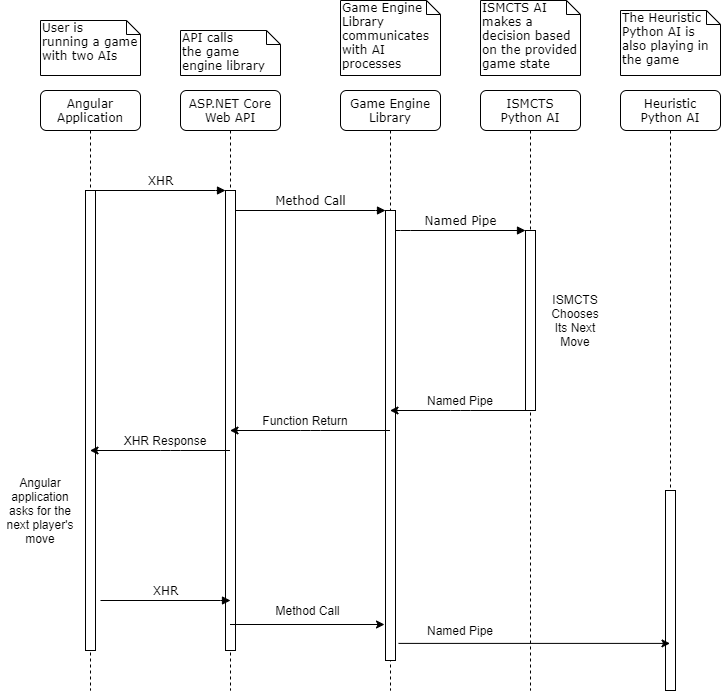
\includegraphics[width=130mm]{colonizers-sequence}}}
\caption{\emph{Colonizers} sequence diagram.}\label{dd:sequence}
\end{figure}

The aforementioned components will be discussed in more detail in the following subsections.

\subsection{Game Engine}

This subsection will discuss not only the C\# library implementing the game logic,
but also the ASP.NET Core Web API, since the library is provided to the user Interface
through Web API calls.

\subsubsection{ASP.NET Core Web API}

The Web API consists of controllers, which define REST (Representational
State Transfer) API endpoints. These endpoints are then called by the Angular
application. In order to promote code reusability, functionality was extracted
from controller methods into separate services, which perform more complex operations
such as formulating method calls to the game engine. The following controllers
are present in the project (in the \texttt{Controllers} directory at the top level
of the project directory):
\begin{itemize}
    \item \texttt{GameController} is responsible for manipulating game state.
        It contains endpoints for creating new games, performing actions during
        gameplay, and for cleaning up after a game is finished.
    \item \texttt{AIController} provides methods for configuring the AI
        scripts in \emph{Colonizers} --- it facilitates adding new AIs
        and changing the Python executable path used to execute AI scripts.
\end{itemize}

The following services are present in the Web API project (in the \texttt{Services}
directory at the top level of the project directory):
\begin{itemize}
    \item \texttt{FileDialogService} uses the Electron API to open
        file dialogs. These are used to select AIs to add and to
        configure the Python executable path.
    \item \texttt{GameService} makes calls to the game engine library.
        It is responsible for configuring and managing.
    \item \texttt{PlayerService} is responsible for the creation of player
        objects. Since there are three different types of players
        in \emph{Colonizers} (human player, AI script player and an AI folder player),
        their creation is not trivial. Therefore this logic was extracted to this
        service.
    \item \texttt{PythonExecutableService} is responsible for managing
        the path to the used Python executable. Selecting the path every
        time the application restarts would be very inconvenient, therefore
        the application remembers the configured path. This path is stored
        in on disk in the game's installation folder.
    \item \texttt{StateService} only serves to store game state information
        in between API calls from the UI application. This avoids
        unnecessary transfer of JSON data containing the entire game
        state with every API call.
\end{itemize}

The ASP.NET Core Web API also sets up DI (dependency injection) for both itself and
the game engine. ASP.NET Core provides its own DI framework
which is used in this application. The DI is configured in the
\texttt{ConfigureServices} method of the \texttt{Startup} class.
The game engine provides an extension method \texttt{AddColonizersGame}
for easy registration of all its components into DI.

\subsubsection{Game Engine Library}
\label{subsub:gelibrary}

All game logic is implemented in the \texttt{Game} C\# library. This
makes game logic a reusable unit, which was useful during the implementation of
the experiment project.

First, we will discuss the representation of game state. The root
of the model class hierarchy is the \texttt{GameState} class, shown in \Cref{dd:gamestate}.
This class may be found in the root of the \texttt{Game} project.

\begin{figure}[ht]
\begin{code}[commandchars=\\\{\},codes={\catcode`\$=3\catcode`\^=7\catcode`\_=8}]
/// <summary>
/// Indicates whether the game is over in this state
/// </summary>
public bool GameOver $\{$ get; set; $\}$ = false;

/// <summary>
/// If the game is over, contains game results
/// </summary>
public GameEndInfo GameEndInfo $\{$ get; set; $\}$

/// <summary>
/// The state of the game board
/// </summary>
public BoardState BoardState $\{$ get; set; $\}$

/// <summary>
/// Things the current player can do on their turn
/// </summary>
public IList<IGameAction> Actions $\{$ get; set; $\}$
\end{code}
\caption{GameState class from the game engine library.}\label{dd:gamestate}
\end{figure}

This object represents all game state data during a single game of \texttt{Colonizers}.
Therefore it (or modified versions of it) is used for communicating the game state
to other components, be it the UI or AI scripts. Note that it also contains information
about whether the game ended and how it ended. Lastly, it also contains a list of possible
actions that could be taken from the current game state. This allows AIs to easily
work with the game state without having to worry about enumerating the action
space themselves. We also include a simplified version of the \texttt{BoardState} class
for reference,
since it contains all data concerned with the actual state of the board, as seen
in \Cref{dd:boardstate}. This class is also located in the root folder
of the \texttt{Game} project.

\begin{figure}[ht]
\begin{code}
    public enum Phase { ColonistPick, Draw, Discard, Power, Build }
    public IList<PlayerInfo> Players { get; set; }
    public IReadOnlyList<Colonist> PlayableColonists { get; set; }
    public IList<Colonist> AvailableColonists { get; set; }
    public List<Module> Deck { get; set; }
    public IReadOnlyList<Module> StartingDeck { get; set; }
    public IList<Module> DiscardTempStorage { get; set; }
    public int PlayerTurn { get; set; }
    public Phase GamePhase { get; set; }
\end{code}
\caption{BoardState model class (simplified).}\label{dd:boardstate}
\end{figure}

A noteworthy property of the \texttt{BoardState} class is \texttt{DiscardTempStorage}.
This property is used to temporarily hold modules after a player has chosen to draw
modules from the deck, but before they have decided which one to keep.

Another interesting part of the game engine is the way the game logic is implemented.
The game has multiple turns in every round and multiple phases in each turn,
organized in a way that resembles a state machine. Maintaining such a class hierarchy
would not be a viable strategy, since cyclic references would be an inevitability.
In order to avoid dependency hell and make the code structure easier to maintain
and understand, we have employed the mediator pattern, facilitated by the
\texttt{MediatR} library. This allows us to separate logic pertaining
to particular game phases into their own, self-contained units without complicated
external dependencies. The game logic classes are separated into three categories:
\begin{itemize}
    \item \texttt{Commands} --- the basic models of actions to perform on
        a particular board state. Every kind of action taken by players in the game
        has its own \texttt{Command} associated with it, marked by the
        \texttt{IGameAction} interface. These commands may be dispatched via
        the mediator. They are located in the \texttt{Commands} directory.
    \item \texttt{CommandHandlers} --- classes which implement logic mutating
        the game board. For example, if we have a command representing the action
        of building a module, a \texttt{BuildModule} command will be dispatched
        via the mediator, and then handled by the \texttt{BuildModuleCommandHandler}.
        Command handlers only mutate the game state based on their input command,
        they do not enumerate possible actions. They are located in the
        \texttt{CommandHandlers} directory.
    \item \texttt{ActionGetters} --- these classes are responsible for
        enumerating the actions space. They receive an input game state,
        and from it they generate a list of actions which are legal
        in this state. They are located in the \texttt{ActionGetters} directory.
\end{itemize}

Each \texttt{CommandHandler} has a reference to its associated \texttt{ActionGetters}.
If we imagine this situation in a state machine context, the \texttt{CommandHandlers}
handle movement between states, and \texttt{ActionGetters} are responsible for
finding out which states we can move to next afterwards. The whole game logic
system consists of pure classes and functions, meaning for the same input,
they provide the same output. This is a crucial property of this design,
considering the game logic is quite complex in certain places. It gives the code
consistency between runs, and makes it easy to debug and understand.

We can examine a high-level method which processes a single turn of the game
in \Cref{dd:engineturn}. We can see that given a game state and a list of players,
we first ask the current player to choose a move. After they have selected
a move, the appropriate \texttt{Command} is passed into the game logic
structure through the mediator. The structure then returns a new game state
along with a list of actions possible in this new state.

\begin{figure}[ht]
\begin{code}
public async Task<GameState> ProcessTurn(GameState gameState, 
    IReadOnlyList<IPlayer> players)
{
    var boardState = gameState.BoardState;
    IPlayer currentPlayer = players[boardState.PlayerTurn - 1];
    int moveId = await currentPlayer.GetMove(gameState, resolver);
    var selectedMove = gameState.Actions[moveId];
    return await resolver.Resolve(selectedMove);
}
\end{code}
\caption{Processing of a single game turn.}\label{dd:engineturn}
\end{figure}

Lastly, the game engine library contains the code responsible for communicating
with the Python AI implementations. This communication is done
via named pipes. When a game is starting, a named pipe is created for each
AI. The AI is then started as a separate process using the configured
Python executable path. This process is passed its pipe name
as an argument. When the AI starts up, it connects to the pipe and starts listening.
The game engine will send a request for a decision to be made, and the AI may
start deciding. When the AI chooses a move, the move is returned through
the same pipe. The pipe is also used for other communication between
the AI and the game engine, notably for requesting determinization and
simulating moves. It is worth mentioning that due to the fact that
the named pipes have pre-defined names, it is not currently possible
to run multiple instances of the game on the same machine. We say currently,
since implementing a mechanism for randomizing the pipe names would
not be a very complicated extension of the library.

\subsection{User Interface}

\emph{Colonizers} uses Electron as a means to run the game as a desktop application,
since the game is developed using web technologies. Specifically, it uses the
Electron.NET library, which provides an access to the Electron APIs to C\# applications,
and it also facilitates usage of Electron's build tools to package C\# applications.
C\# and the whole .NET platform in general still do not have a widely-used cross-platform
UI framework, therefore Electron was a good fit for this project.

The UI for \emph{Colonizers} is an Angular application, which is then served inside
Electron. This application is located in the \texttt{ClientApp} directory
in the \texttt{Desktop} project directory.
Electron then uses the Chromium rendering engine and Node.js in the background.
The Angular application allows configuration of the game, it handles presentation
of game state to the user, and it is responsible for communicating with the
ASP.NET Core Web API.

In order to do development work on the UI, it is recommended that you use
Visual Studio 2019. It has a very useful feature whereby it allows you to debug
both JavaScript and C\# code at the same time in the same project. Since the Angular
application is located in the same project as the Web API, this is an invaluable
feature. Since the UI is an Angular application, naturally it is possible
to run and debug it without running it in Electron. The source code for this project
contains launch settings pre-configured for Visual Studio 2019 in order to accomplish
exactly this. A sidenote is that while running outside Electron, the application
does not have access to Electron APIs. \emph{Colonizers} uses the File Dialog
API multiple times, therefore this functionality will be unavailable in this case.
Interaction with the Electron APIs is always preceded by a check whether
the application instance is running inside Electron, therefore calls
to methods which use Electron APIs will not cause exceptions. We can see
such a guard for Electron presence in \Cref{dd:electronguard}.

It is also possible to debug the application while it is running inside Electron.
The command \texttt{electronize start} will launch the application
inside Electron when run. It is then possible to attach to the application's
process in Visual Studio 2019. This allows us to debug code which uses Electron
API calls, which is not possible when not running in Electron. The mentioned
command also has a useful option --- \texttt{electronize start /watch}
which will watch application files
for changes and re-compile only changed application files.

\begin{figure}[ht]
\begin{code}[commandchars=\\\{\},codes={\catcode`\$=3\catcode`\^=7\catcode`\_=8}]
public async Task<bool> AddSingleScript()
$\{$
    if (HybridSupport.IsElectronActive)
    $\{$
        BrowserWindow mainWindow = Electron.WindowManager
            .BrowserWindows.First();
        OpenDialogOptions options = new OpenDialogOptions
        $\{$
            Properties = new OpenDialogProperty[] $\{$
                    openDialogProperty
                $\}$
        $\}$;

        string[] files = await Electron.Dialog.ShowOpenDialogAsync(
            mainWindow, options);
    $\}$

    return false;
$\}$
\end{code}
\caption{Electron API call guarded by check for Electron presence.}\label{dd:electronguard}
\end{figure}

The source code for the Angular application is written in TypeScript, CSS and HTML.
The HTML used is not pure HTML, rather the HTML files are Angular templates.
Angular Templates are a way to insert data into markup seamlessly.
The TypeScript files are transpiled to JavaScript at build-time.
We use Angular in a client-side mode, whereby the source files are compiled
ahead of time, and are delivered to the client on-demand. Angular also
offers a server-side rendering option, allowing to offload some work
from clients onto servers. However, due to the fact that both client and server
run on the same machine in \emph{Colonizers}, this option was not used.

The most important building blocks of Angular are \emph{Components}.
Components control the view presented to the user, and they prepare
data for presentation by the view. We can see the source code for a component
in \Cref{dd:componentcode}

\begin{figure}[ht]
\begin{code}[commandchars=\\\{\},codes={\catcode`\$=3\catcode`\^=7\catcode`\_=8}]
@Component($\{$
    selector: 'app-discard',
    templateUrl: './discard.component.html',
    styleUrls: ['./discard.component.css']
$\}$)
export class DiscardComponent implements OnInit $\{$

    @Input() gameState: GameState;
    @Output() onPick = new EventEmitter<number>();

    constructor() $\{$ $\}$

    ngOnInit() $\{$
    $\}$

    getModules(): Module[] $\{$
        // Find the appropriate modules in the temp discard storage
        return this.gameState.actions.map(
            x => this.gameState.boardState.discardTempStorage
                .find(y => y.name === x.module));
    $\}$

    keep(module: Module) $\{$
        this.onPick.next(this.gameState.actions.findIndex(
            x => x.module == module.name));
    $\}$

$\}$
\end{code}
\caption{An Angular component.}\label{dd:componentcode}
\end{figure}

We can see a few important component features in \Cref{dd:componentcode}:
\begin{itemize}
    \item The definition of the component's template and styles
        in the \texttt{@Component} decorator. Notably, the styles
        specified in this scope only apply to this component's
        template.
    \item The component has an \texttt{@Input()} and an \texttt{@Output()}.
        These are the ways other components interact with this one.
        Keeping component interaction to only inputs and outputs makes
        components pure, meaning they will output the same data
        when provided with the same inputs. In a complex application,
        this is a very desirable property, since it makes debugging
        easier and bugs more rare.
    \item The component defines a selector --- \texttt{app-discard}.
        Using this selector, other components can include this one in
        their templates.
\end{itemize}

We can see an example of the aforementioned component being used in \Cref{dd:componentref}.
The excerpt is from \texttt{GameComponent}'s template, and it demonstrates how
it binds one of its own fields as an input for the \texttt{DiscardComponent},
and that it is listening for events emitted by it.

\begin{figure}[ht]
\begin{code}[commandchars=\\\{\},codes={\catcode`\$=3\catcode`\^=7\catcode`\_=8}]
<div *ngIf="isWaitingForHumanPlayer && isDiscardPhase()">
    <app-discard [gameState]="gameState"
                 (onPick)="onHumanPlayerAction(\$event)">
    </app-discard>
</div>
\end{code}
\caption{Usage of Angular component in another component's template.}\label{dd:componentref}
\end{figure}

These features are the core of how the UI application is built --- it is based on
a~divide-and-conquer principle, where the entire view is composed of smaller components,
which are in turn composed of even smaller components.

Another notable building block of \texttt{Colonizers} is the usage of Angular
services. A service in Angular is meant to be a way to abstract data manipulation
and API calls away from components. Therefore, all code pertaining to
communication with the ASP.NET Core Web API is contained within
the two service classes --- \texttt{GameService} and \texttt{ScriptsService}.

\subsection{AI framework}

In the previous subsection, we have already discussed the communication between
game engine and the AI from the game engine's point of view. In this subsection,
we will examine the other side. The API provided to AIs is contained
within the \texttt{AICore.py} source file (located in the root folder of the
\texttt{AICore} project), in the abstract class \texttt{AIBase}.
This class is meant to be a base class for all AI implementations
added to the game. It provides the AIs with the following functionality:
\begin{itemize}
    \item Communication with the game engine. The AIs do not need to
        manually read from and write to pipes, this is handled by base
        class methods. Whenever the game engine requests an action from the
        AI, the base class will read this message from the named pipe, and invoke
        the AI code to get a response. It then writes this response back to the
        named pipe.
    \item Other communication with the game engine --- determinization
        and simulation. Determinization, provided a game state with hidden
        information, will produce a game state with perfect information. This
        is done by the game engine using information set data it tracks
        internally. This is used in algorithms like ISMCTS or our adapted
        version of MaxN, both of which we examined in the experimental
        part of this thesis.
    \item The \texttt{AICore.py} source file also contains various
        utility functions for working with game state.
        Game state is provided to AIs as a dictionary which
        copies the structure of the \texttt{GameState}
        object we discussed in \Cref{subsub:gelibrary}.
        Among these functions are utilities like counting
        modules in a player's colony on a per-color basis.
\end{itemize}

Since the game engine executes the AIs by running them from the command line
with a Python interpreter, it is crucial that the \texttt{AICore.py}
file be accessible to them. To this end, whenever an AI is added to the game,
it is copied into a folder in the game files containing the \texttt{AICore.py}
file. With folder-based AIs the situation is a little more tricky, since
importing files higher in a folder hierarchy is not straightforward in Python.
Therefore, when copying in folder-based AIs, a copy of \texttt{AICore.py}
is copied along with the new files into the new folder. This way, the AI
has access to this file at runtime.

Observe that during application build or publish, the AIs which ship with
the game are copied into the publish folder. This is accomplished through
the .csproj files for the \texttt{Desktop} and \texttt{Experiments} projects.

While creating AIs for the game, debugging the AI is relatively straightforward.
Simply set a breakpoint at the game engine location where the AI is being
run with the Python interpreter, then skip the line creating the actual process
and instead run your own process in debug mode in your development environment
of choice.

The following is a description of the API provided by the \texttt{AIBase}
class:
\begin{itemize}
    \item \texttt{messageCallback(self, gameState)} --- abstract method, must be implemented
        in descendants. This method is called by the framework when it is the AI's
        turn in the game, and its response is required. The gameState object represents
        the current game state (the object will be described later in this section).
        The expected return value is a string containing a single number,
        corresponding to the index of the chosen action. The by index we mean the zero-based
        index of the chosen action in the \texttt{gameState["Actions"]} list.
    \item \texttt{determinize(self)} --- uses the information set stored by the game
        engine to produce a determinized version of the current game state.
        The return value is the determinized version with all hidden information
        revealed.
    \item \texttt{simulate(self, boardState, move)} --- simulates the given move
        on the given board state, and returns the new game state. The \texttt{move}
        parameter must be a string representation of an action, following the specific
        format returned by the \texttt{getActionString(action)} function
        of the \texttt{AICore.py} file.
    \item \texttt{run(self, pipeName)} --- initializes the communication
        with the game engine. The \texttt{pipeName} parameter is passed to the AI
        script as the only argument, therefore it is located at \texttt{sys.argv[1]}
        in the main AI file. A typical usage pattern is shown in \Cref{dd:airun}
\end{itemize}

\begin{figure}[ht]
\begin{code}[commandchars=\\\{\},codes={\catcode`\$=3\catcode`\^=7\catcode`\_=8}]
if \_\_name\_\_ == "\_\_main\_\_":
    ai = ISMCTS\_AI() \# Inherits from AIBase
    ai.run(sys.argv[1])
\end{code}
\caption{Common usage scenario of the \texttt{run(self, pipeName)} method.}
\label{dd:airun}
\end{figure}

There are a number of other utility functions in the \texttt{AICore.py} file,
however most of them are not worth mentioning here, since they are simply one line
shorthands for common operations. There is one worth mentioning however ---
\texttt{getActionString(action)}. This function converts an action (as obtained from
the \texttt{gameState["Actions"]} list) into the shorthand string format
used by the \texttt{simulate(self, boardState, move)} method.

\subsubsection{Issues with embeddable Python}
\label{dd:embedpy}

Embeddable versions of Python ignore \texttt{PYTHONPATH}, and this causes issues
when running AI scripts. To avoid this issue, either use a regular Python installation,
or add the lines shown in \Cref{dd:embedex} to the top of your AI script.
However, editing the scripts in the aforementioned way sometimes still does not fix the issue.
The only sure way to get rid of the problem is to use a regular Python installation.

\begin{figure}[ht]
\begin{code}[commandchars=\\\{\},codes={\catcode`\$=3\catcode`\^=7\catcode`\_=8}]
import sys
sys.path += '.'
\end{code}
\caption{Workaround for issues with embeddable Python installations.}
\label{dd:embedex}
\end{figure}

\subsection{Experiments}
\label{chap:experimentdocs}

The experiments performed in this thesis are implemented in the \texttt{Experiments}
project of the \texttt{Colonizers} solution. It is a C\# console application project.
It is invoked via the command line with two arguments --- the first is a~number
between 1 and 5, corresponding to the experiment number, and the second
is the path to the Python executable to use when executing AI scripts.
Note that the attachments to this thesis do not contain a binary
for the \texttt{Experiments} project, therefore you will have to build and
run it yourself. This may be done by installing the required software for
developing \emph{Colonizers} mentioned in this chapter, navigating to the
\texttt{Experiments} project folder, and running the command \texttt{dotnet run},
followed by the parameters required by the program.

After the experiment is run, it will produce a JSON file containing the results
of the experiment. This file is generated in the directory where the \texttt{Experiments}
project is run from.
\Cref{dd:experimentjson} shows the structure of these JSON files, with less
important fields omitted for brevity. The JSON files associated with the five
experiments are also located in the \texttt{Results} folder of the \texttt{Experiments}
project. They were added there for reference, since
some experiments may take tens of hours to run even on reasonably fast
machines. Be aware that a simple diff of the JSON result files
is not sufficient for determining whether or not a given experiment was successfully
replicated. This is because the files contain running times of the games as well.

\begin{figure}[ht]
\begin{code}[commandchars=\\\{\},codes={\catcode`\$=3\catcode`\^=7\catcode`\_=8}]
$\{$
    "Players": [
        "Name": "ISMCTS",
        "PlayerEndInfo": $\{$
            "Ranking": 3,
            "VictoryPoints": 24,
            "Player": $\{$
                "ID": 1,
                ...
            $\}$
        $\}$
    ],
    "Duration": "00:12:28.1879334"
$\}$
\end{code}
\caption{Experiment result JSON file structure (simplified).}\label{dd:experimentjson}
\end{figure}

The class \texttt{Scenarios} contains the configuration and setup for the experiments,
and each scenario then calls \texttt{ExperimentRunner} to performed
the experiment itself. There is no need to configure anything more than
passing the program the required parameters, the experiment scenarios
are set up exactly as they were performed by the author.

A noteworthy point is the implementation of the shuffling of players between games.
Since the game engine already possessed an implementation of the Fisher-Yates Shuffle
\cite{Knuth98} for shuffling lists, this implementation was reused for shuffling the
players themselves. This means that if we were to run the experiments
without shuffling, and instead assigning the players the same positions they would
have been assigned by the shuffle, the results of this experiment would be different.
This is because running the shuffle manipulates the game engine's random number generator.
